% !TeX root = ./cj-2020-kesskiessburkstoeck.tex
%%
%% This is file `sample-sigchi.tex',
%% generated with the docstrip utility.
%%
%% The original source files were:
%%
%% samples.dtx  (with options: `sigchi')
%% 
%% IMPORTANT NOTICE:
%% 
%% For the copyright see the source file.
%% 
%% Any modified versions of this file must be renamed
%% with new filenames distinct from sample-sigchi.tex.
%% 
%% For distribution of the original source see the terms


%% for copying and modification in the file samples.dtx.
%% 
%% This generated file may be distributed as long as the
%% original source files, as listed above, are part of the
%% same distribution. (The sources need not necessarily be
%% in the same archive or directory.)
%%
%% The first command in your LaTeX source must be the \documentclass command.
\documentclass[sigchi, nonacm=true]{acmart}
\usepackage{subfigure}
\usepackage{nth}
\usepackage{booktabs}
% \usepackage{todonotes}
%%
%% \BibTeX command to typeset BibTeX logo in the docs
\AtBeginDocument{%
  \providecommand\BibTeX{{%
    \normalfont B\kern-0.5em{\scshape i\kern-0.25em b}\kern-0.8em\TeX}}}

%% Rights management information.  This information is sent to you
%% when you complete the rights form.  These commands have SAMPLE
%% values in them; it is your responsibility as an author to replace
%% the commands and values with those provided to you when you
%% complete the rights form.
\setcopyright{acmcopyright}
\copyrightyear{2020}
\acmYear{2020}
% \acmDOI{10.1145/1122445.1122456}

%% These commands are for a PROCEEDINGS abstract or paper.
\acmConference[Computational Journalism Symposium '20]{Computational Journalism Symposium '20}{March 20--21, 2020}{Boston, MA}
\acmBooktitle{Boston '20: Computational Journalism Symposium,
  March, 20--21, 2020, Boston, MA}
% \acmPrice{15.00}
% \acmISBN{978-1-4503-XXXX-X/18/06}


%%
%% Submission ID.
%% Use this when submitting an article to a sponsored event. You'll
%% receive a unique submission ID from the organizers
%% of the event, and this ID should be used as the parameter to this command.
%%\acmSubmissionID{123-A56-BU3}

%%
%% The majority of ACM publications use numbered citations and
%% references.  The command \citestyle{authoryear} switches to the
%% "author year" style.
%%
%% If you are preparing content for an event
%% sponsored by ACM SIGGRAPH, you must use the "author year" style of
%% citations and references.
%% Uncommenting
%% the next command will enable that style.
%%\citestyle{acmauthoryear}

%%
%% end of the preamble, start of the body of the document source.
\begin{document}

%%
%% The "title" command has an optional parameter,
%% allowing the author to define a "short title" to be used in page headers.
\title[Partisan and News Content]{Partisan and News Content on YouTube during 2019 Federal State Elections in Germany}

%%
%% The "author" command and its associated commands are used to define
%% the authors and their affiliations.
%% Of note is the shared affiliation of the first two authors, and the
%% "authornote" and "authornotemark" commands
%% used to denote shared contribution to the research.
\author{Philipp Kessling}
% \authornote{Both authors contributed equally to this research.}
\email{philipp.kessling@haw-hamburg.de}
\orcid{1234-5678-9012}
\affiliation{%
  \institution{HAW Hamburg, Department of Information}
  \streetaddress{Finkenau 35}
  \city{Hamburg}
  \state{Germany}
  \postcode{22081}
}

\author{Bastian Kiessling}
% \authornote{Both authors contributed equally to this research.}
\email{bastian.kiessling@haw-hamburg.de}
\orcid{1234-5678-9012}
\affiliation{%
  \institution{HAW Hamburg, Department of Information}
  \streetaddress{Finkenau 35}
  \city{Hamburg}
  \state{Germany}
  \postcode{22081}
}
\author{Steffen Burkhardt}
% \authornote{Both authors contributed equally to this research.}
\email{steffen.burkhardt@haw-hamburg.de}
\orcid{1234-5678-9012}
\affiliation{%
  \institution{HAW Hamburg, Department of Information}
  \streetaddress{Finkenau 35}
  \city{Hamburg}
  \state{Germany}
  \postcode{22081}
}
\author{Christian St\"ocker}
% \authornotemark[1]
\email{christian.stoecker@haw-hamburg.de}
\affiliation{%
  \institution{HAW Hamburg, Department of Information}
  \streetaddress{Finkenau 35}
  \city{Hamburg}
  \state{Germany}
  \postcode{22081}
}

%%
%% By default, the full list of authors will be used in the page
%% headers. Often, this list is too long, and will overlap
%% other information printed in the page headers. This command allows
%% the author to define a more concise list
%% of authors' names for this purpose.
\renewcommand{\shortauthors}{Kessling et al.}

%%
%% The abstract is a short summary of the work to be presented in the
%% article.
\begin{abstract}
  YouTube has emerged as one of the most commonly used platforms for entertainment, information and political communication, for media consumers as well as professional communicators. News organizations and political parties alike have adopted strategies for publishing video content–ranging from already broadcasted news programs to political speeches of local party members. In this ongoing study we interrogate YouTube ranking algorithm on the occasions of three federal state elections in Germany. We retrieved ranked search results for every parties leading candidate in the elections, as well as the comments and replies which YouTube determines as relevant for each video occurring in the rankings. Preliminary results show that content dealing with and content authored by far-right parties is most widely consumed and interacted with. The ranking of the content is relatively stable over time but partially interrupted by short phases that jumble the previous order.
\end{abstract}

%%
%% The code below is generated by the tool at http://dl.acm.org/ccs.cfm.
%% Please copy and paste the code instead of the example below.
%%
% \begin{CCSXML}
% <ccs2012>
%  <concept>
%   <concept_id>10010520.10010553.10010562</concept_id>
%   <concept_desc>Computer systems organization~Embedded systems</concept_desc>
%   <concept_significance>500</concept_significance>
%  </concept>
%  <concept>
%   <concept_id>10010520.10010575.10010755</concept_id>
%   <concept_desc>Computer systems organization~Redundancy</concept_desc>
%   <concept_significance>300</concept_significance>
%  </concept>
%  <concept>
%   <concept_id>10010520.10010553.10010554</concept_id>
%   <concept_desc>Computer systems organization~Robotics</concept_desc>
%   <concept_significance>100</concept_significance>
%  </concept>
%  <concept>
%   <concept_id>10003033.10003083.10003095</concept_id>
%   <concept_desc>Networks~Network reliability</concept_desc>
%   <concept_significance>100</concept_significance>
%  </concept>
% </ccs2012>
% \end{CCSXML}

% \ccsdesc[500]{Computer systems organization~Embedded systems}
% \ccsdesc[300]{Computer systems organization~Redundancy}
% \ccsdesc{Computer systems organization~Robotics}
% \ccsdesc[100]{Networks~Network reliability}

%%
%% Keywords. The author(s) should pick words that accurately describe
%% the work being presented. Separate the keywords with commas.
\keywords{Political Communication, YouTube, partisan and news content}


%%
%% This command processes the author and affiliation and title
%% information and builds the first part of the formatted document.
\maketitle

\section{Introduction}

  In line with the increasing use of social media services in the political landscape \cite{silber_social_2016}, YouTube has become a platform for political information and campaigns during elections periods. Parties and politicians can thus reach the public without dependency on the gatekeeping function of traditional mass media. News organizations have also adopted to the affordance of the service to distribute their content, trying to build up an online audience \cite{al_nashmi_promoting_2017}. This study is focusing on the ranking and consumption of videos retrieved in connection with three federal state elections in Germany. It examines the impact of content produced by parties and news media and the influence of YouTube’s ranking algorithm in a political context. Finally, the study aims at explaining the distribution of party and media content as well as the related interaction of users and patterns within the ranking system.


\subsection{YouTube and Political Communication}
  % Role of YouTube
  YouTube is a platform for news, information, entertainment and especially social interaction \cite{khan_social_2017}. It is the most relevant video-sharing platform worldwide -- n western Europe it is even more popular than Facebook \cite{silber_social_2016}.
  According to YouTube, users watch over a billion hours of video and generate billions of views every day. More than 1.9 billion registered users visit the platform every month. More than 70\% of the traffic now comes from mobile devices \cite{youtube_youtube_2019}. YouTube is also among the most popular social media services in Germany. 40\% of the entire population use the video sharing platform at least once a week. Young people, 14 to 29 years old, are leading users-metrics with an overall weekly activity share of 92\% \cite{ard_ard/zdf-onlinestudie_2019}.
  
  Participatory engagements appear as click-based interactions, e.g. likes, shares and comments. Consuming videos or reading comments are classified as passive engagements \cite{khan_social_2017}. Although YouTube was initially implemented as a service for user-generated content, it was quickly adopted by actors with commercial interests \cite{castells_communication_2007} as wells as public service broadcasters \cite{iosifidis_public_2011}. Both, user-generated content and professionally created videos are now actively watched and shared \cite{xu_networked_2016}. The distribution of views can be described with the \textit{Pareto principle} \cite{cha_i_2007}: the most viewed, most popular videos account for the vast majority of views while majority of the content is barely noticed.

  Political parties use YouTube to spread their agenda, addressing the users of the video-sharing service circumventing traditional media channels. % without dependency
  The platform is an additional communication channel with increasing relevance for political actors \cite{johann_durchdachte_2018}. A direct form of communication is possible due to opportunities for self-expression and interaction. Social media such as YouTube are used as additional tools that extend traditional campaigning \cite{carlson_riding_2008, gibson_normalising_2015}. In Germany, many politicians do not operate their own YouTube channels. In most cases, videos are published by the respective party channels to reach a wider audience \cite{schweitzer_normalization_2011}.
  
  By showcasing leadership, they predominantly use the platform for positive campaigning by expressing an optimistic vision instead of depreciating political opponents \cite{sohal_content_2018}. 
 
  % News organizations
  News organizations have also taken to making use of the opportunities provided by YouTube to distribute their content \cite{bruns_gatewatching:_2005}. After considering what news are most appropriate for their agenda, a proportion of their news coverage in featured on YouTube. Media use YouTube to extend their traditional distribution channels. There appears to be focus on items that can be labeled as ‘hard news’ such as reports about politics \cite{al_nashmi_promoting_2017}. There is a controversial scientific discourse about the impact of social media services on democratic processes in the society: Some argue that social media has weakened the gatekeeper role in favor of user-powered communities \cite{bruns_gatewatching:_2005}. In this scenario, highly rated news is prominently featured while unpopular content stays widely unnoticed. Others stress that existing elites have quickly adapted to these disruptive technologies and thus increased their status of dominance \cite{kperogi_cooperation_2011}. According to \cite{dylko_filtering_2012}, popular political news on YouTube feature elites, are created by elites, and predominantly consist of traditional media content.

  % Research object
  \subsection{The impact of the ranking algorithm}
    Regarding YouTube’s ranking algorithm, the order of videos in the search results cannot simply be linked to interaction metrics such as likes, comments and view count \cite{rieder_ranking_2018}.
    The authors of the study discovered three patterns of ordering: (1) a stable ranking over a long period of time, which is characterized by very little variation within the top ranked videos, (2) a relatively stable ranking with, what the authors call, newsy \textit{newsy} interruptions \cite[p. 63]{rieder_ranking_2018} on specific days and (3) strong variations in the top-most ranks over time. The study further shows that a given video´s upload date is a crucial factor for said video´s rank stability. Old videos are stable in rank, whereas newly uploaded content changes its position in the search ranking very quickly. Another analysis in this field has revealed that top ranked videos usually have a higher position stability, while videos from active users are more highly ranked than videos from trustworthy sources \cite{fernandez-llatas_are_2017}. This complements findings, according to which the ranking algorithm favors content from niche channels even if their videos received fewer views than major mainstream channels \cite{rieder_ranking_2018}.

  \section{Research Question}
    This study connects the interaction metrics of video content published by news media and political parties in election times with YouTube’s ranking algorithm. Not only the sources of videos will be considered for the analysis, but also differences and patterns for videos related to each leading candidate of involved parties. We therefore propose the following research questions:
    \begin{description}
      \item[RQ1] Which candidate’s search results score the highest accumulated consumptions statistics, especially video views and comments?
      \item[RQ2] Which patterns can be observed in the video ranking system for leading candidates during elections?
    \end{description}

\section{Method and Data Retrieval}

  The study analyzes YouTube content regarding three federal state elections in Germany which were held on \nth{1} September 2019 in Brandenburg and Saxony as well as on October \nth{27} in Thuringia.
  Several similarities stand out when comparing the elections results. First, the Alternative for Germany (AfD), a far-right political party, with their leading candidates Andreas Kalbitz in Brandenburg, J\"org Urban in Saxony and Bj\"orn H\"ocke in Thuringia, became the second-strongest party in all federal state parliaments–this represents a massive leap in comparison to the party’s results in 2014, see table \ref{tbl::electionres}. Second, the Christian Democratic Union (CDU), liberal-conservative, and the Social Democratic Party (SPD), social-democratic, remained the strongest party in each of their ruling states despite an ongoing downward slide. The Left (Die Linke), democratic-socialist, additionally emerged as the largest party in Thuringia but slipped in both other states. The Green Party, usually weak in eastern Germany, gained votes in Brandenburg and Saxony while staying on the same level in Thuringia. Notably, the FDP (liberal-democrats) returned to the state parliament in Thuringia, while it failed to clear the 5-percent hurdle in Brandenburg and Saxony.
 
  % latex table generated in R 3.6.1 by xtable 1.8-4 package
  % Fri Feb 14 11:20:48 2020
  \begin{table*}[t!]
    \centering
    \begin{tabular}{llll}
      \toprule
      Party & Thuringia & Saxony & Brandenburg \\ 
      \midrule
      Die Linke & Bodo Ramelow & Rico Gebhardt & Kathrin Dannenberg \\ 
      CDU & Mike Mohring & Michael Kretschmer & Ingo Senftleben \\ 
      SPD & Wolfgang Tiefensee & Martin Dulig & Dietmar Woidke \\ 
      AfD & Bj\"orn H\"ocke & J\"org Urban & Andreas Kalbitz \\ 
      Grüne & Anja Siegesmund, & Katja Meier & Ursula Nonnemacher, \\
      &  Dirk Adams & & Benjamin Raschke \\
      FDP & Thomas Kemmerich & Holger Zastrow & Peter Goetz \\ 
      Freie W\"ahler &  &  & Péter Vida \\ 
      \bottomrule
    \end{tabular}

    \caption{The full name of each of these leadings candidates were used as search term.}
    \label{tbl::searchterms}
  \end{table*}

   Our analysis aims at directly answering the research questions: Using 12-hour intervals, we retrieved the relevance ranked search results with a maximum of 50 items per iteration for all 21 relevant leading candidates in the three elections. The candidates’ names were used as the search term. This retrieval process has started in August 2019 and is currently ongoing–the analysis in this study is based on preliminary data extending to early November 2019. Accessing YouTube's search API endpoint\footnote{See \url{https://developers.google.com/youtube/v3/docs/search/list}.} with multiple accounts, we retrieve a relevance-ranked search result and give each item a number according to its position in the search result list. For each entry in the search result we also retrieve consumption statistics (included are count of views, likes, dislikes and comments). In order to exclude YouTube's search personalization bias the study was conducted with multiple newly generated accounts.
  We accumulate the consumption statistics YouTube delivers with every video object. We utilize a variant of the RankFlow plots employed in \cite{rieder_ranking_2018} to visualize ranking and video consumption over time.
  Videos are posted by channels, we gather a list of distinct channels in the data set and execute a preliminary coding of these channels into the following categories: party-affiliated, news organization-affiliated and other channels.
  
  % > filter(
  % +     search2,
  % +     between(
  % +         scrapedAt,
  % +         as.POSIXct("2019-08-01"),
  % +         as.POSIXct("2019-11-30")
  % +     )
  % + ) %>% distinct(id.videoId) %>% nrow()
  % [1] 1965

  So far, 1,965 distinct videos were gathered and considered for this preliminary analysis. Excluded from our analysis were videos by channels, that bore no connection to the German political landscape. This included six individual videos from channels belonging to musicians and comedians, in detail: Trap God, Ingo ohne Flamingo, Freshtorge, Coldplay, a n d s y, JohannesOerdingVEVO.

\section{Discussion}

  \begin{figure}[]
    \centering
    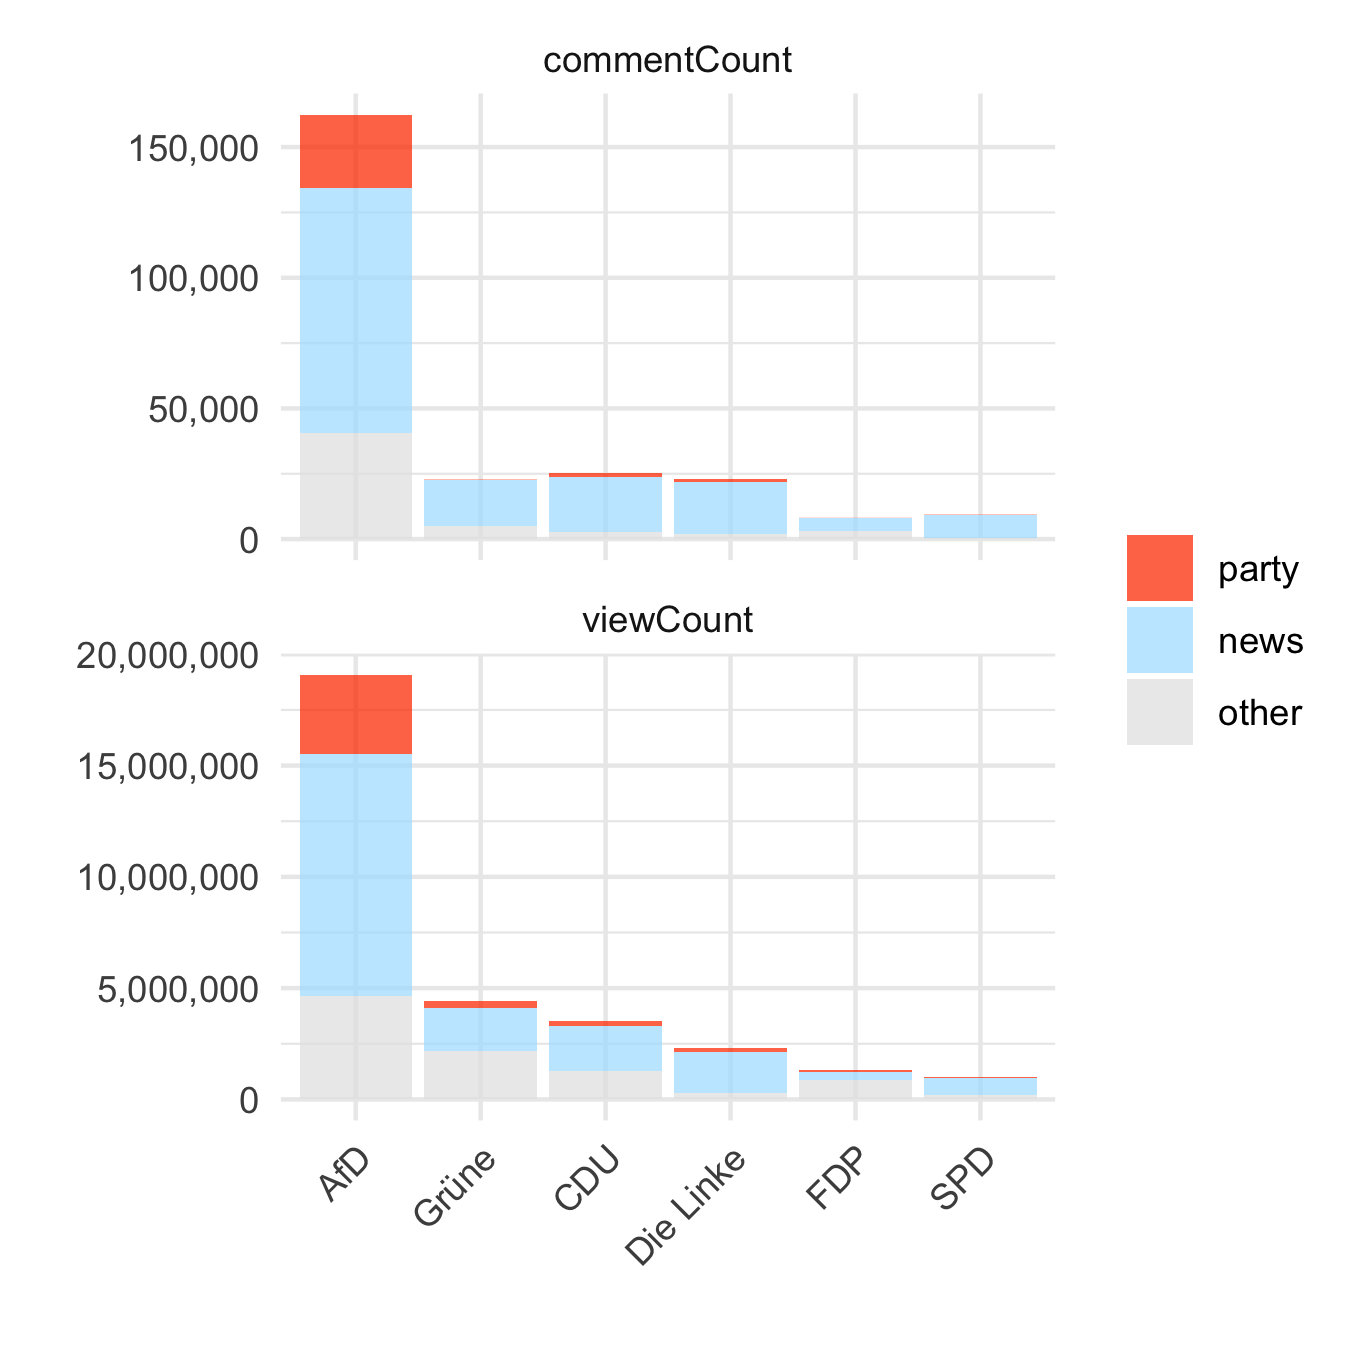
\includegraphics[width=\linewidth]{plots/combined.png}

    \caption{Cumulated number of comments and views per unique video. Calculation in based on YouTube's consumption statistics, for multiple instances of one video per candidate the metrics mean was utilized.}
    \label{fig::comment_count}
  \end{figure}

  % Comment count
  As shown in Figure \ref{fig::comment_count}, videos uploaded in connection with the AfD politicians Bj\"orn H\"ocke, Andreas Kalbitz and J\"org Urban gained most user comments in the data set. Additionally, the content created by this party initiated more active debates in comparison to all other parties in the sample. Comments were strongly focused on content provided by media channels, except for AfD content.
  A small number of videos accumulated the vast majority of comments.

  % latex table generated in R 3.6.1 by xtable 1.8-4 package
  % Wed Feb 12 10:45:19 2020
  \begin{table}[h]
    \centering

    \begin{tabular}{lrrr}
      
      \multicolumn{4}{c}{\textbf{Results 2019}} \\
      \toprule
      Party & Saxony & Thuringia & Brandenburg \\ 
      \midrule
      CDU & 32.1\% & 21.7\% & 15.6\% \\ 
      Die Linke & 10.4\% & 31.0\% & 10.7\% \\ 
      SPD & 7.7\% & 8.2\% & 26.2\% \\ 
      AfD & 27.5\% & 23.4\% & 23.5\% \\ 
      Gr\"une & 8.6\% & 5.2\% & 10.8\% \\ 
      FDP & 4.5\% & 5.01\% & 4.1\% \\ 
      \bottomrule\\
      
      \multicolumn{4}{c}{\textbf{Comparison to 2014}} \\
      \toprule
      Party & Saxony & Thuringia & Brandenburg \\ 
      \midrule
      CDU & -7.3\% & -11.8\% & -7.4\% \\ 
      Die Linke & -8.5\% &  2.8\% & -7.9\% \\ 
      SPD & -4.6\% & -4.2\% & -5.7\% \\ 
      AfD &  17.7\% &  12.8\% &  11.3\% \\ 
      Gr\"une &  2.9\% & -0.5\% &  4.6\% \\ 
      FDP &  0.7\% &  2.5\% &  2.6\% \\ 
      \bottomrule
    \end{tabular}

    \vspace{0.25cm}
    \caption{Election results for each of the three German federal states held in 2019 and discussed in this study. \cite{der_landeswahlleiter_fur_brandenburg_brandenburger_nodate, statistisches_landesamt_des_freistaates_sachsen_wahlergebnisse_nodate, thuringer_landesamt_fur_statistik_wahlen_nodate}}
    \label{tbl::electionres}
  \end{table}

  \begin{figure*}[t!]
    \centering
    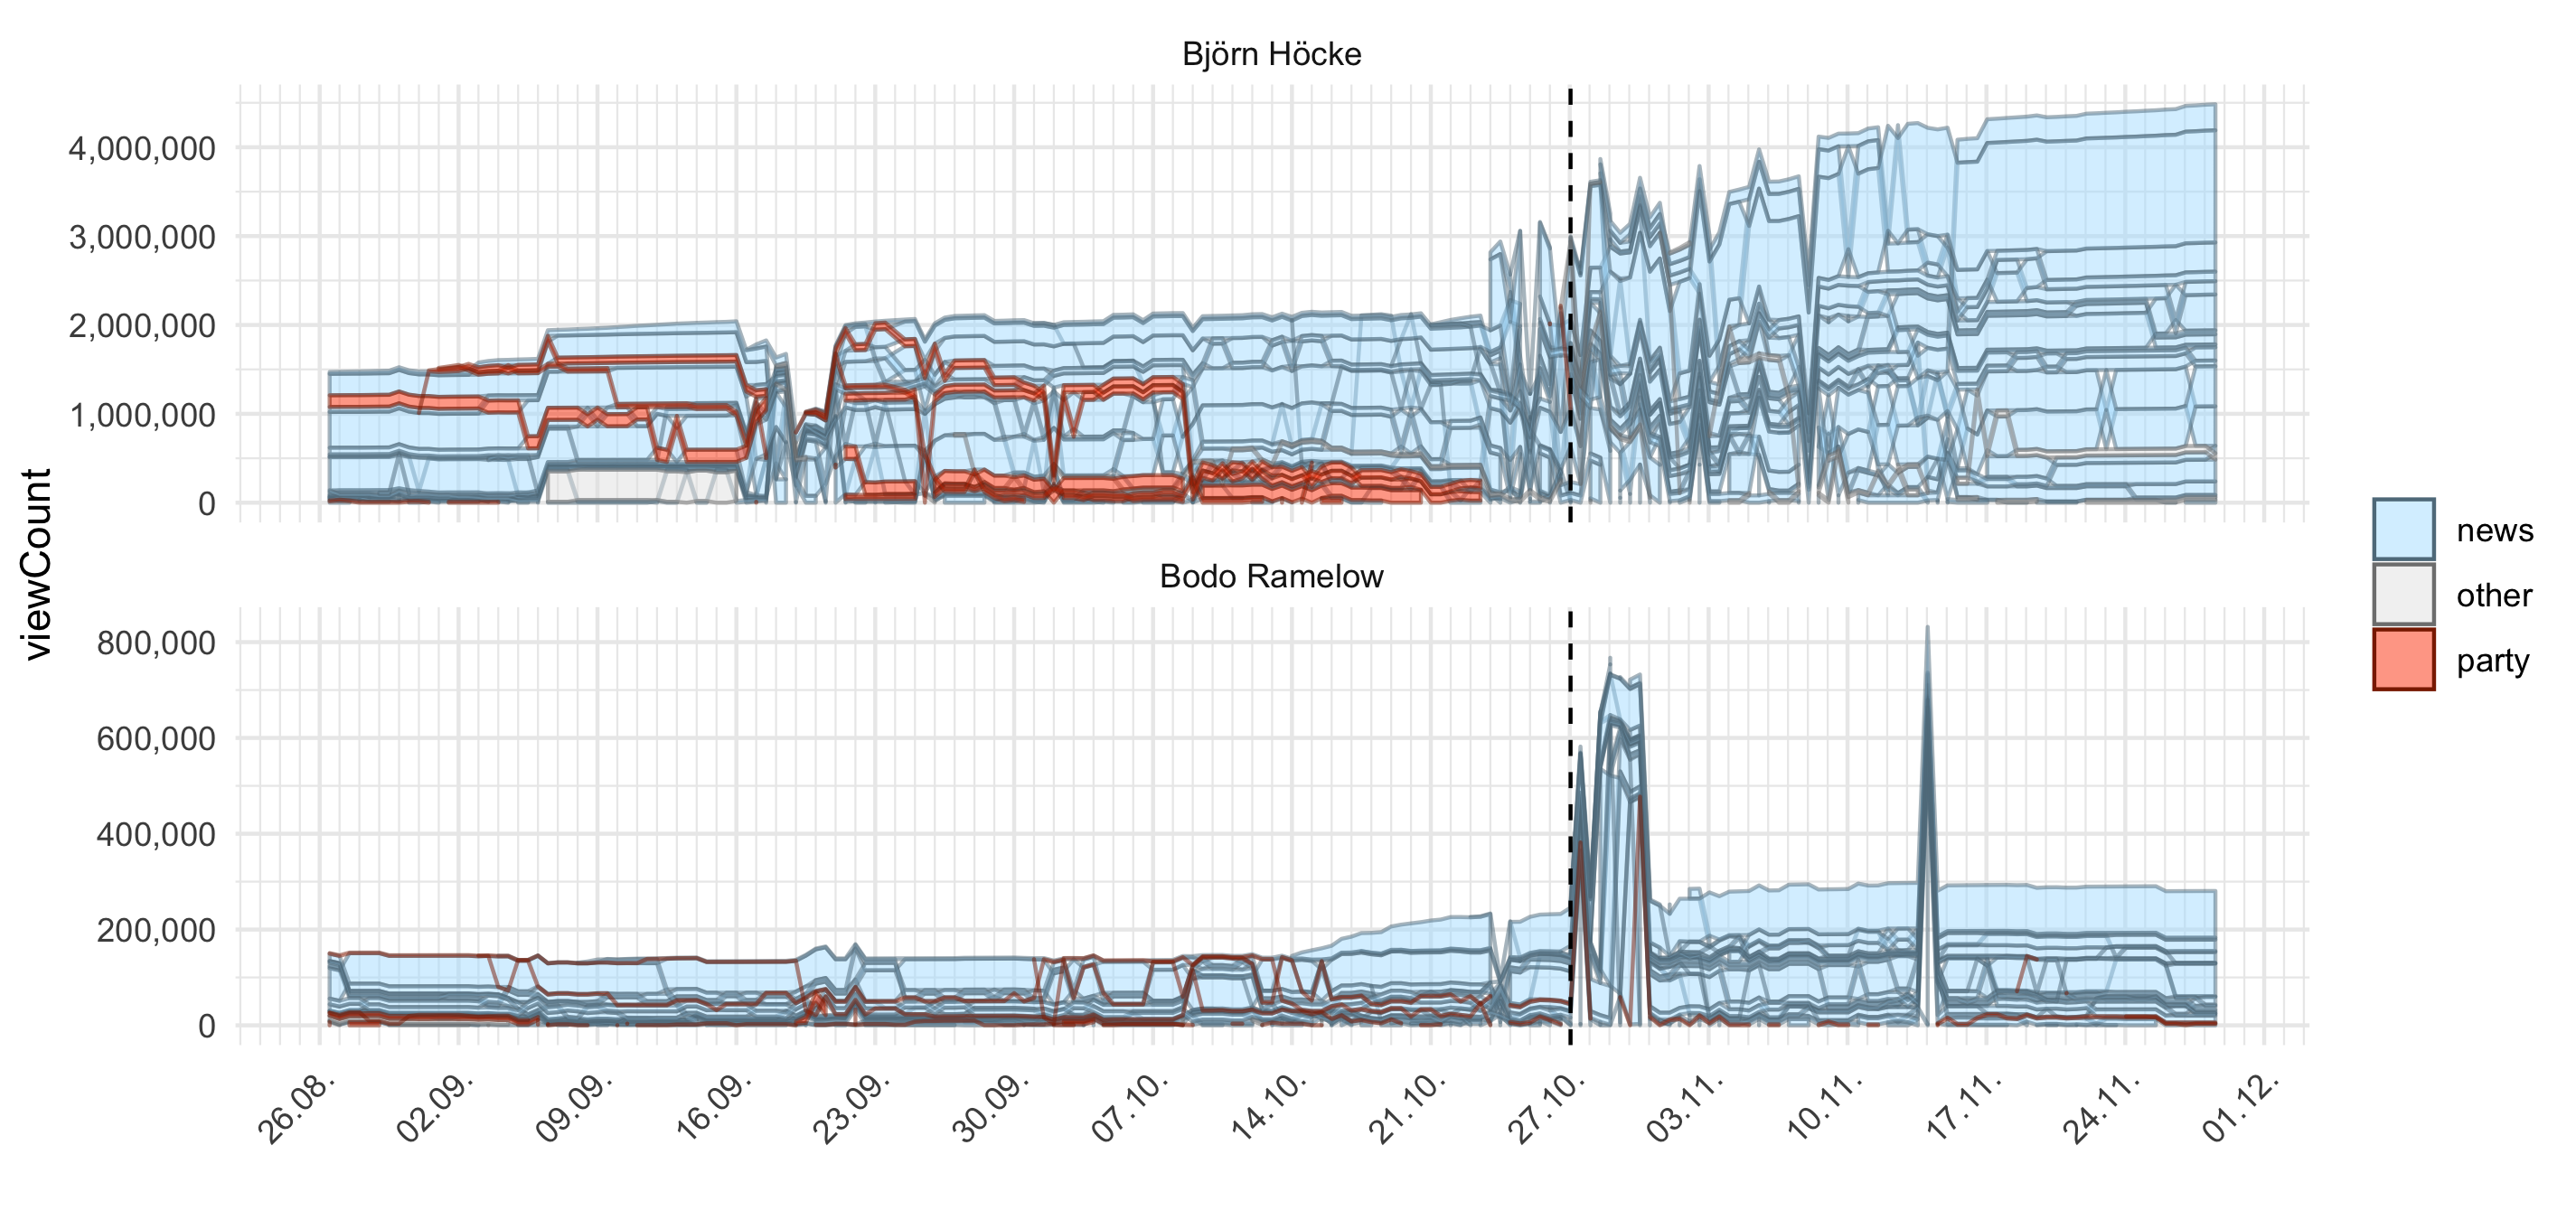
\includegraphics[width=0.9\fulltextwidth]{plots/ranked_rameow_hoecke.png}

    \caption{Example of RankFlow plots for two Thuringian candidates: colour represent source affiliation, the vertical order represents the rank. For clarity only the top 20 ranked videos are displayed. Dashed black line indicates the election day in Thuringia, \nth{27} October.}
    \label{fig::rankflows}
  \end{figure*}

  % View Count
  Figure \ref{fig::comment_count} illustrates the accumulated view and comment count for each party in the research sample. The data clearly shows that videos in connection with the AfD candidates Bj\"orn H\"ocke, Andreas Kalbitz and J\"org Urban, were most watched and interacted with, followed at some distance by content mentioning candidates of The Greens. The majority of parties did not generate a significant impact on YouTube.
  Some of the disparities between the results for the three AfD candidates can be explained by Bj\"orn H\"ocke’s special role inside the party: He is widely perceived (even though that is not an elected post) as one of the leaders of the so-called “Fl\"ugel” (translated \textit{"wing"}), a far-right group inside the party proper. This group has been declared suspect of pursuing goals contrary to the German constitution by Germany’s internal intelligence agency, the \textit{Verfassungsschutz} \cite{bundesamt_fur_verfassungschutz_fachinformation_2019}. The “Fl\"ugel” and its leading figure H\"ocke are thus subject to a disproportionate amount of news reporting.

  Figure \ref{fig::rankflows} shows the ranking order for videos uploaded in relation to Bj\"orn H\"ocke and Bodo Ramelow, both contenders in the federal state election in Thuringia. The ranking is relatively stable with newsy interruptions, a result similar to those observed by \cite{rieder_ranking_2018} in another context. During this phase new videos quickly arise, jumbling the previous ranking system, while also gaining views over time. This is most prominently visible in the vicinity of the election day -- the \nth{27} October 2019. Another observation is the rapid gain (and in the case of Bodo Ramelow, equally rapid loss) of momentary view counts cooccuring with the advent of elections results and the connected news reporting.

  The question why content connected with far-right figures, such as H\"ocke or Kalbitz is consumed in larger volume than content of moderate and mainstream figures remains open and is subject to future research. Although it invites speculation, we assume a higher interest in controversial debates -- which are more likely to emerge in the vicinity of controversial figures.

\section{Conclusion}

  In this study, we have retrieved and analyzed relevance-ranked search results and comment lists for 21 candidates in three federal state elections in Germany in 2019. Our goal was to find ways in which (a) gatekeeper content on the one hand, and (b) party-affiliated content, on the other, is weighted and ranked. Furthermore, we aimed at finding in which ways users interact with the found content.
  
  Our findings suggest greater interactivity on and consumption of content reporting about far-right politicians compared to mainstream politicians. With the exception of content authored by the AfD, party-affiliated content did receive a smaller share of views. This pattern is also found in the user commenting behavior: Far-right party-affiliated videos receive the largest share of comments while mainstream party-affiliated generates muss less interaction. Again, comments on videos from news organizations again show a discrepancy between news and party affiliated content. Regarding the ranking systems, the analysis reveals relatively stable ranks over time for most of the candidates interrupted by so-called newsy patterns, in which videos climb and fall within the ranking in a short period of time. 
  
  In conclusion, the data shows that the AfD has implemented an effective social media communication strategy on YouTube by providing content that is actively watched and commented on. For all other leading candidates from relevant parties in the campaigning process, news videos dominated YouTube content judging by view count and comments. Stable ranking patterns dominate in the observed period of time, interrupted by rapid but intense changes in the ranking system that correlates with relevant political developments during elections and especially the actual election day. The data leads to the assumption that content from far-right parties generates more attention in social media in general. However, it does not provide any information on the factor of attention, generated by views and comments that are connotated positively or negatively. Therefore, a further analysis should examine the sentiment and possibly other features of the content itself.
  
%%
%% The acknowledgments section is defined using the "acks" environment
%% (and NOT an unnumbered section). This ensures the proper
%% identification of the section in the article metadata, and the
%% consistent spelling of the heading.
\begin{acks}
  The authors acknowledge support by the German Federal Ministry of Education and Research (FKZ 16KIS0752) and thank the reviewers for their most helpful comments.
\end{acks}

%%
%% The next two lines define the bibliography style to be used, and
%% the bibliography file.
\bibliographystyle{ACM-Reference-Format}
\bibliography{literature}

%%
%% If your work has an appendix, this is the place to put it.
\appendix

\end{document}
\endinput
